\section{Evaluation}
\label{sec:experiment}


In this section, we compare the optimized SGEMM performance in Gflop/s with NVIDIA cuBLAS. 
Our SGEMM achieves $17\%\sim 25\%$ performance
improvement, which confirms the usefulness of the microarchitectural optimization on GPU. 
We present 
a quantitative analysis of the effect of each optimization strategy and an estimation of the upper bound performance using a roofline model.

The experiments are conducted on NVIDIA K20m GPU with its hardware configuration summarized in 
Table~\ref{table:k20}. We compare with cuBLAS from CUDA $7.0$. In our experiments, we choose square matrices for $A$, $B$
and $C$, and  the matrix sizes vary from $384$ to $12288$ with a step $384$.
%\jled{C size? What about A and B?}

\begin{table}[htbp]
\caption{The specification of NVIDIA Tesla K20m GPU.}
\centering
\scalebox{0.8} {
\begin{tabular}{|c|c|}
\hline
% Metric& Value\\
Configuration& Value\\
\hline
SPs/SM &192\\
\hline
SMs&13\\
\hline
Cores &2496\\
\hline
Frequency&705 MHz\\
\hline
Memory Bus Width&320 bit \\
\hline
Memory frequency&2600 MHz\\
\hline
Bandwidth&208.0 GB/s\\
\hline
Peak GFlop/s in SP&3520 Gflop/s\\
\hline
Warp scheduler per SM&4\\
\hline
Dispatch unit/SM&8\\
\hline
Max Registers/thread&256 \\
\hline
    32-bit registers/SM&65536 \\ %\jled{Use actual number}\\
\hline
LD/ST unit&32 \\
\hline
shared memory size&48KB\\
\hline
L1 cache size&16 or 48 KB\\
\hline
L2 cache size&1536 KB\\
\hline
\end{tabular}
}
\label{table:k20}
\end{table}


\subsection{Overall Performance}
Figure~\ref{fig:sgemm_tn} reports the performance of cuBLAS SGEMM and our optimized SGEMM.
When matrix size is $12288\times12288$, the optimized SGEMM achieves $3104$
GFlop/s with $88\%$ efficiency, while cuBLAS gets $2705$ GFlop/s with $76\%$ efficiency.
Our SGEMM achieves $3104/2705=1.15X$ speedup in performance improvement over cuBLAS.% $12\%$ in efficiency.

The overall trend in Figure~\ref{fig:sgemm_tn} is that SGEMM performance increases with matrix sizes. 
%\jled{the next sentence change to ``On the one hand, a larger matrix has a higher arithmetic intensity 9$AI$), which is the ratio of compulsory floating-point operations to the total DRAM memory traffic.
%The high arithmetic intensity makes good use of GPU computing resources to obtain good performance.''}
For one thing, a large matrix has a high ratio of 
floating-point operations to the store operations of matrix $C$, which is more close to the hardware arithmetic intensity. 
For anther, a larger matrix has a better load balance on GPU by increasing the workload of the threading CUDA
cores.
%\jled{change to ``number of threading blocks''}. 
The number of threading blocks ranges in $2 \times 2, 8 \times 8, \dots, 64 \times 64$ from left to right in Figure~\ref{fig:sgemm_tn}.
% $[768/192,768/192]=[4,4]$ to $[12288/192, 12288/192]$ $=[64,64]$. 
Since Kepler has $13$ SMs in total, matrix $384\times 384$ suffers more from load imbalance because of few ($4$) blocks. 
This is why there is a significant performance growth from $384$ to $1536$ for SGEMM. 
With respect to performance improvement over cuBLAS, our optimizations benefit more on larger matrices. 
The higher arithmetic intensity of larger matrices makes their performance increasingly bounded by the GPU microarchitecture rather than memory. 
Therefore, our microarchitecture-level optimization plays an important role on tuning 
performance.

Figure~\ref{fig:rectangle} shows performance of different matrix shapes. This
also demonstrate our $12\times12$ blocking is better than cuBLAS when matrix greater
than $1000$ and our $8\times8$ blocking implementation, and $8\times8$ blocking
is better than cuBLAS for all shapes. The performance for matrix shape [W, 4W,
W] fluctuates seriously than other shapes, it is because each thread iteration
a longer K=4W than other shapes. The degree of parallelism is coarser than other
three shapes.

\begin{figure}[htbp]
\begin{center}
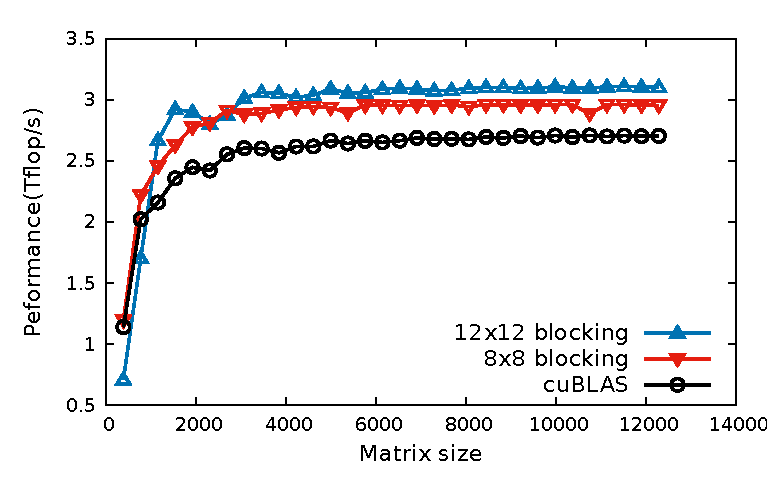
\includegraphics[scale=0.5]{tn_192}
\caption{Performance comparison of CUBLAS and the optimized SGEMM }
\label{fig:sgemm_tn}
\end{center}
\end{figure}


\begin{figure*}
    \begin{subfigure}[htbp]{0.5\textwidth}
        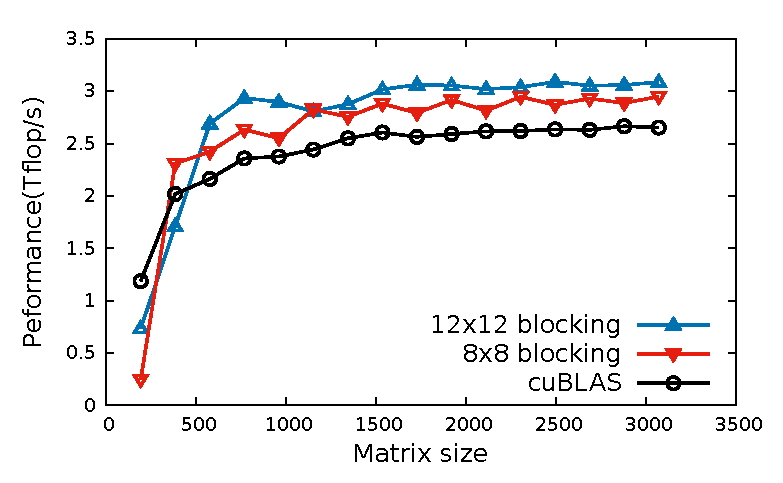
\includegraphics[width=3.0in]{1k2k4k}
        \subcaption{Matrix shape [W, 2W, 4W]}
        \label{fig:control_throughput}
    \end{subfigure}
    %\hspace{20mm}
    \begin{subfigure}[htbp]{0.5\textwidth}
\begin{center}
        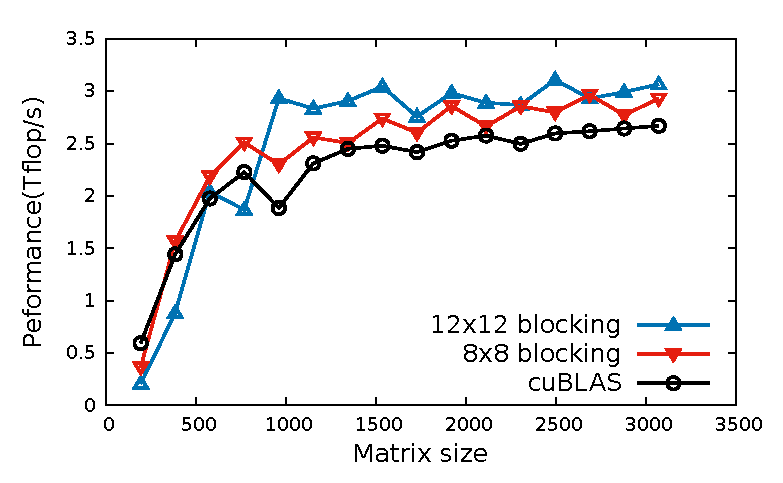
\includegraphics[width=3.0in]{1k4k1k}
\end{center}
        \subcaption{Matrix shape [W, 4W, W]}
        \label{fig:control_latency}
    \end{subfigure}
    \begin{subfigure}[htbp]{0.5\textwidth}
        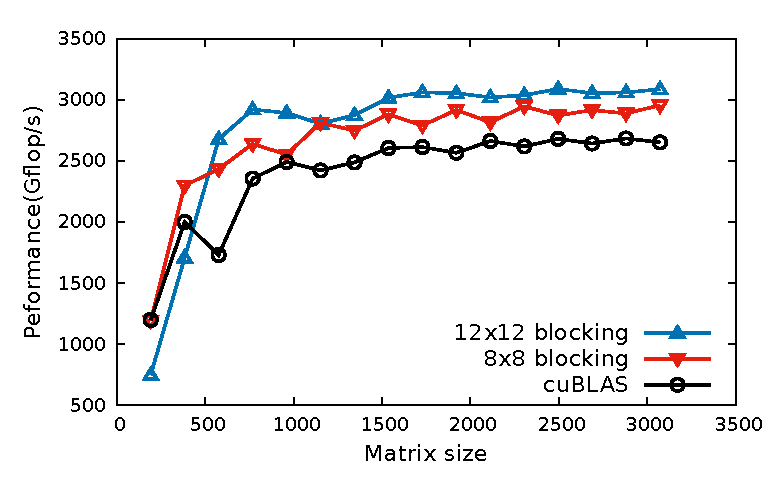
\includegraphics[width=3.1in]{4k1k4k}
        \subcaption{Matrix shape [4W, W, 4W]}
        \label{fig:control_pattern}
    \end{subfigure}
    %\hspace{20mm}
    \begin{subfigure}[htbp]{0.5\textwidth}
        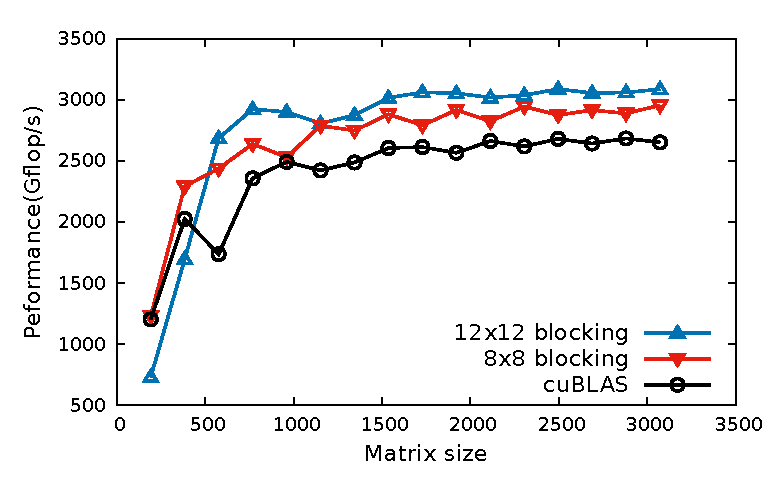
\includegraphics[width=3.1in]{4k2k1k}
        \subcaption{Matrix shape [4W, 2W, W]}
        \label{fig:control_pattern}
    \end{subfigure}
    \caption{Rectangle matrice performance}
    \label{fig:rectangle}
\end{figure*}

\subsection{Performance Analysis}

\subsubsection{the Influence of Register Blocking Size}
Table~\ref{tab:dm} summarizes computation and data movement volume of blocking SGEMM algorithm.
The volume of data moving from shared memory to global memory is $r_x\times b_k+ r_y\times b_k$, and computation volume is $r_x\times r_y\times b_k$. 
The shared memory arithmetic intensity ($sAI$) is defined as the ratio of floating-point operations to the shared memory traffic, which is 
\begin{equation}
sAI = \frac {r_x\times 
r_y\times b_k} {r_x\times b_k+ r_y\times b_k} = \frac{1}{\frac{1}{r_x} + \frac{1}{r_y}}.
    \label{equ:reg_block}
\end{equation}
Register blocking size is limited by the maximal number of registers per thread. 
Each thread needs $r_x\times r_y$, $r_x$ and $r_y$ registers to store the result of a sub-matrix of $C$,  a block-column of
$A$,  a block-row of $B$ in the same loop respectively.
To hide shared memory latency, double-buffered software pipelining is used. Thus, extra $r_x$ and $r_y$ registers
are used to prefetch next block-column of $A$ and $B$ from shared memory. 
Since the total number of registers must be less than the maximal number of registers per thread ($256$ on Kepler), we have
\begin{equation}
    r_x\times r_y + r_x\times 2 + r_y\times 2 < 256.
\label{equ:reg_restrict}
\end{equation}
Equation~\ref{equ:reg_block} implies that larger register blocking yields the higher shared memory arithmetic intensity,
and the optimal solution lies at $r_x=r_y$ with restriction~\ref{equ:reg_restrict}. 
Because data load must be aligned in $128$-bit using 
{\tt LDG.128}, the block size could be $4\times 4$, $8\times 8$ or $12\times 12$. 
Since $4\times 4$ leads to low data reuse in register files, we only show $8\times8$ and $12\times12$ cases in Figure~\ref{fig:sgemm_tn}.
Performance of $12\times12$ is better than $8\times8$ because $12\times12$ blocking has higher $sAI$ and instruction
level parallelism. With respect to 
instruction scheduling optimization in Table~\ref{tab:position}, it has more slots to insert {\tt non-FFMA}
instructions, and latency can be hidden easier.
$12*12+4*12=192$ registers are used by {\tt LD} and {\tt FFMA} instructions, and totally $236$ registers with
other address indices. The number of registers per SM restricts us to launch up to $256$ threads. 
In our implementation, we have $256$ threads per block. 
Each thread block computes a $192\times 192$ sub-matrix of $C$ by multiplying $A_{192,4}$ and $B_{4, 192}$, where $4$ is the unrolling factor.

%\begin{figure}[htbp]
%\begin{center}
%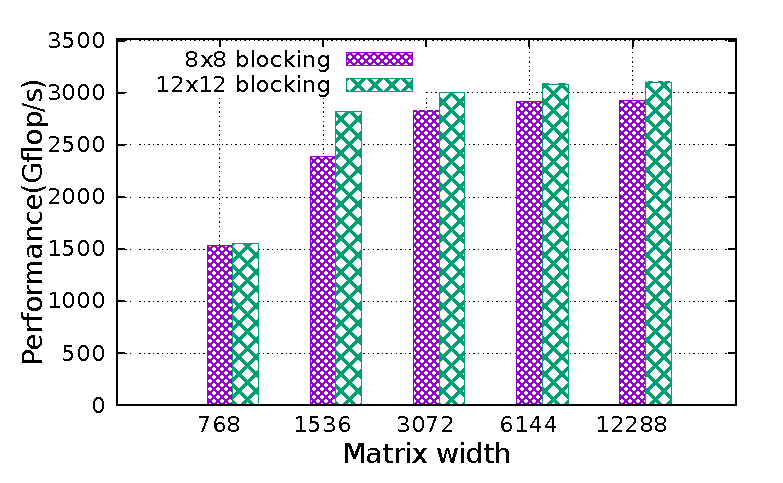
\includegraphics[scale=0.5]{block}
%    \caption{Evaluation of different blocking sizes.} %\jled{could add $4\times4$ case.}}
%\label{fig:block}
%\end{center}
%\end{figure}

Only one thread block per SM is active due to register limitation, thus the thread occupancy is $256/2048=12.5\%$.
With our high instruction level parallelism, the thread parallelism becomes low.
However, our SGEMM's high performance confirms that instruction level parallelism plays an important role on GPU.
The Similar conclusion is mentioned by Volkov in~\cite{volkov2010better}.

\subsubsection{Profiling Microarchitectural Optimization}

To examine performance gain of different optimization strategies, we construct several intermediate 
implementations by incrementally applying our microarchitectural optimizations.
\begin{figure}[htbp]
\begin{center}
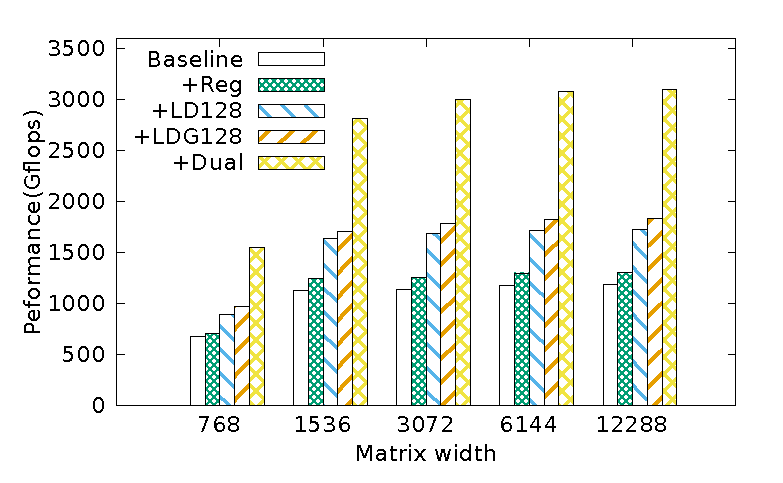
\includegraphics[scale=0.5]{tn_prof}
    \caption{Evaluation of the incremental optimizations.}
\label{fig:th_prof}
\end{center}
\end{figure}

{\it Baseline:}~~The baseline includes conventional optimizations including register blocking, global
memory double buffering, shared memory double buffering and unrolling, without assembly level optimization.
For example, the baseline uses default $32$-bit {\tt LD} rather than $128$-bit {\tt LDG} instruction to load data from global memory.
Registers are allocated orderly first for $C$, from $0$ to $143$, then for $A$ and $B$. 
In this case, {\tt FFMA}s have $368/(144*4)=63.89\%$ 2-way bank conflicts and $64/(144*4)=11.11\%$ 3-way bank conflicts. 
Besides, the baseline cannot apply dual issue optimization either.

{\it +Reg:}~~The register allocation pattern described in section~\ref{sec:register} is applied to eliminate register bank conflict. 
No optimization of instruction scheduling for this version.

{\it +LD128:}~~Use wider global load instruction {\tt LD128} with L2-cached.
Though Kepler has a L1 data cache, it is designed for local rather than global memory access~\cite{gk110}.
% So {\tt LDx} will not be L1-cached, it can be L2-cached.

{\it +LDG128:}~~Use the texture cached {\tt LDG} which is faster than L2-cached {\tt LD}. 
When {\tt LDG} is used, {\tt TEXDEPBAR} is required before the data access due to the weak consistency of texture cache~\cite{lukyanov2014efficient}.

{\it +Dual:}~~Use dual issue control, which is fully enabled by utilizing the pattern described in section~\ref{sec:assembler}.
%Single issue is controlled by setting control code to $0x40$. %\jled{different from section~\ref{sec:benchmark}. The left sentence is useless.}. 
In dual issued mode, {\tt NOP} may be inserted for 7-instruction alignment.

Figure~\ref{fig:th_prof} illustrates performance gains of each optimization method.
As long as the number of instructions changes, rescheduling instruction order is needed to achieve good performance.
Compared to the baseline implementation, SGEMM gains up to $2.6\times$ speedup by applying all the optimizations.
Register bank conflict eliminating improves around $10\%$ performance. 
Wider load instruction {\tt LD128} contributes $27\%-35\%$ performance, texture cached
load instruction {\tt LDG128} improves $5\%-12\%$.
Dual issue achieves the highest improvement, i.e. 84\%-106\%.
%improves the most, $84\%-106\%$.


\begin{figure}[htbp]
\begin{center}
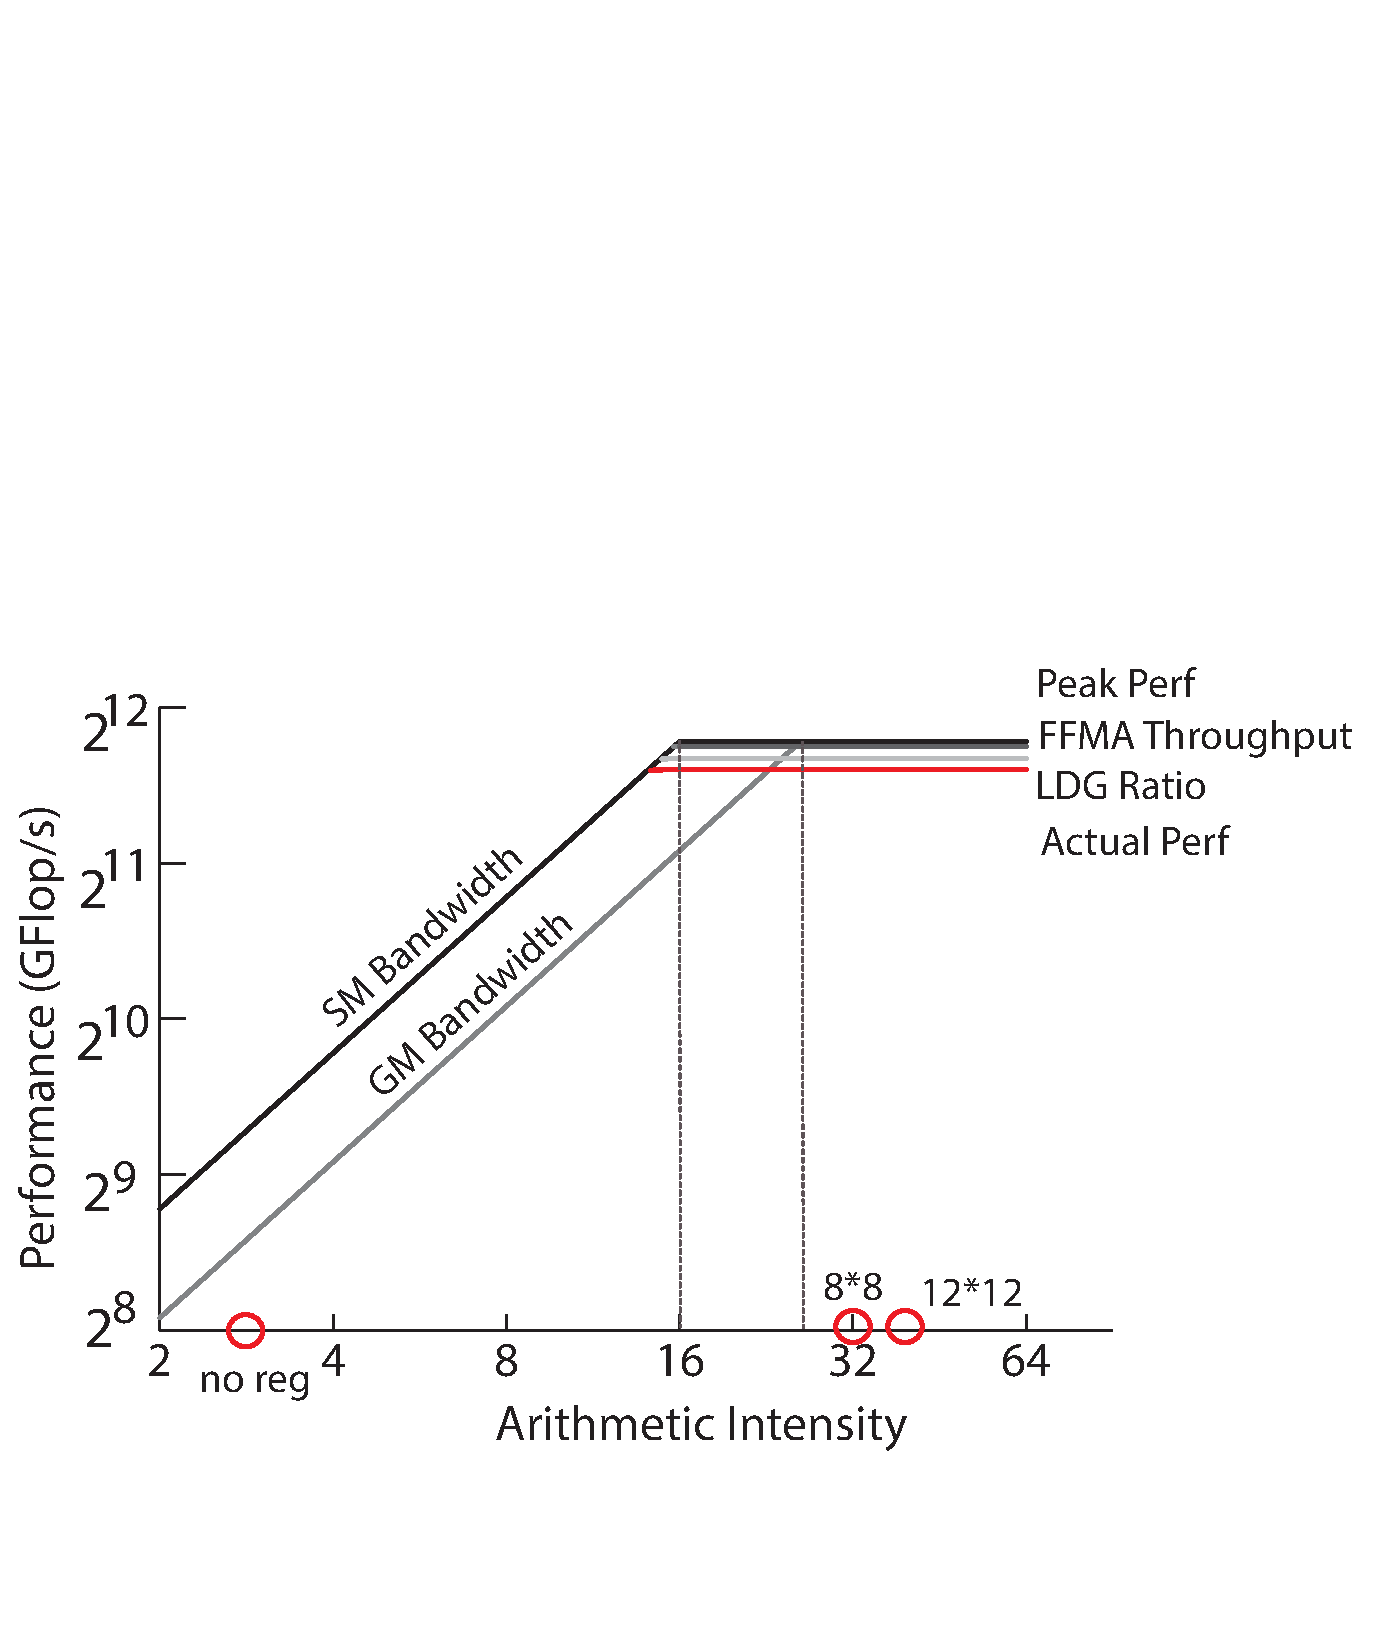
\includegraphics[scale=0.32]{roofline}
    \caption{Global memory roofline model using log-log scale. ``GM Bandwidth'' means global memory's theoretical
    bandwidth.} %Horizontal lines shows different Gflops.}
\label{fig:roofline_global}
\end{center}
\end{figure}

\begin{figure}[htbp]
\begin{center}
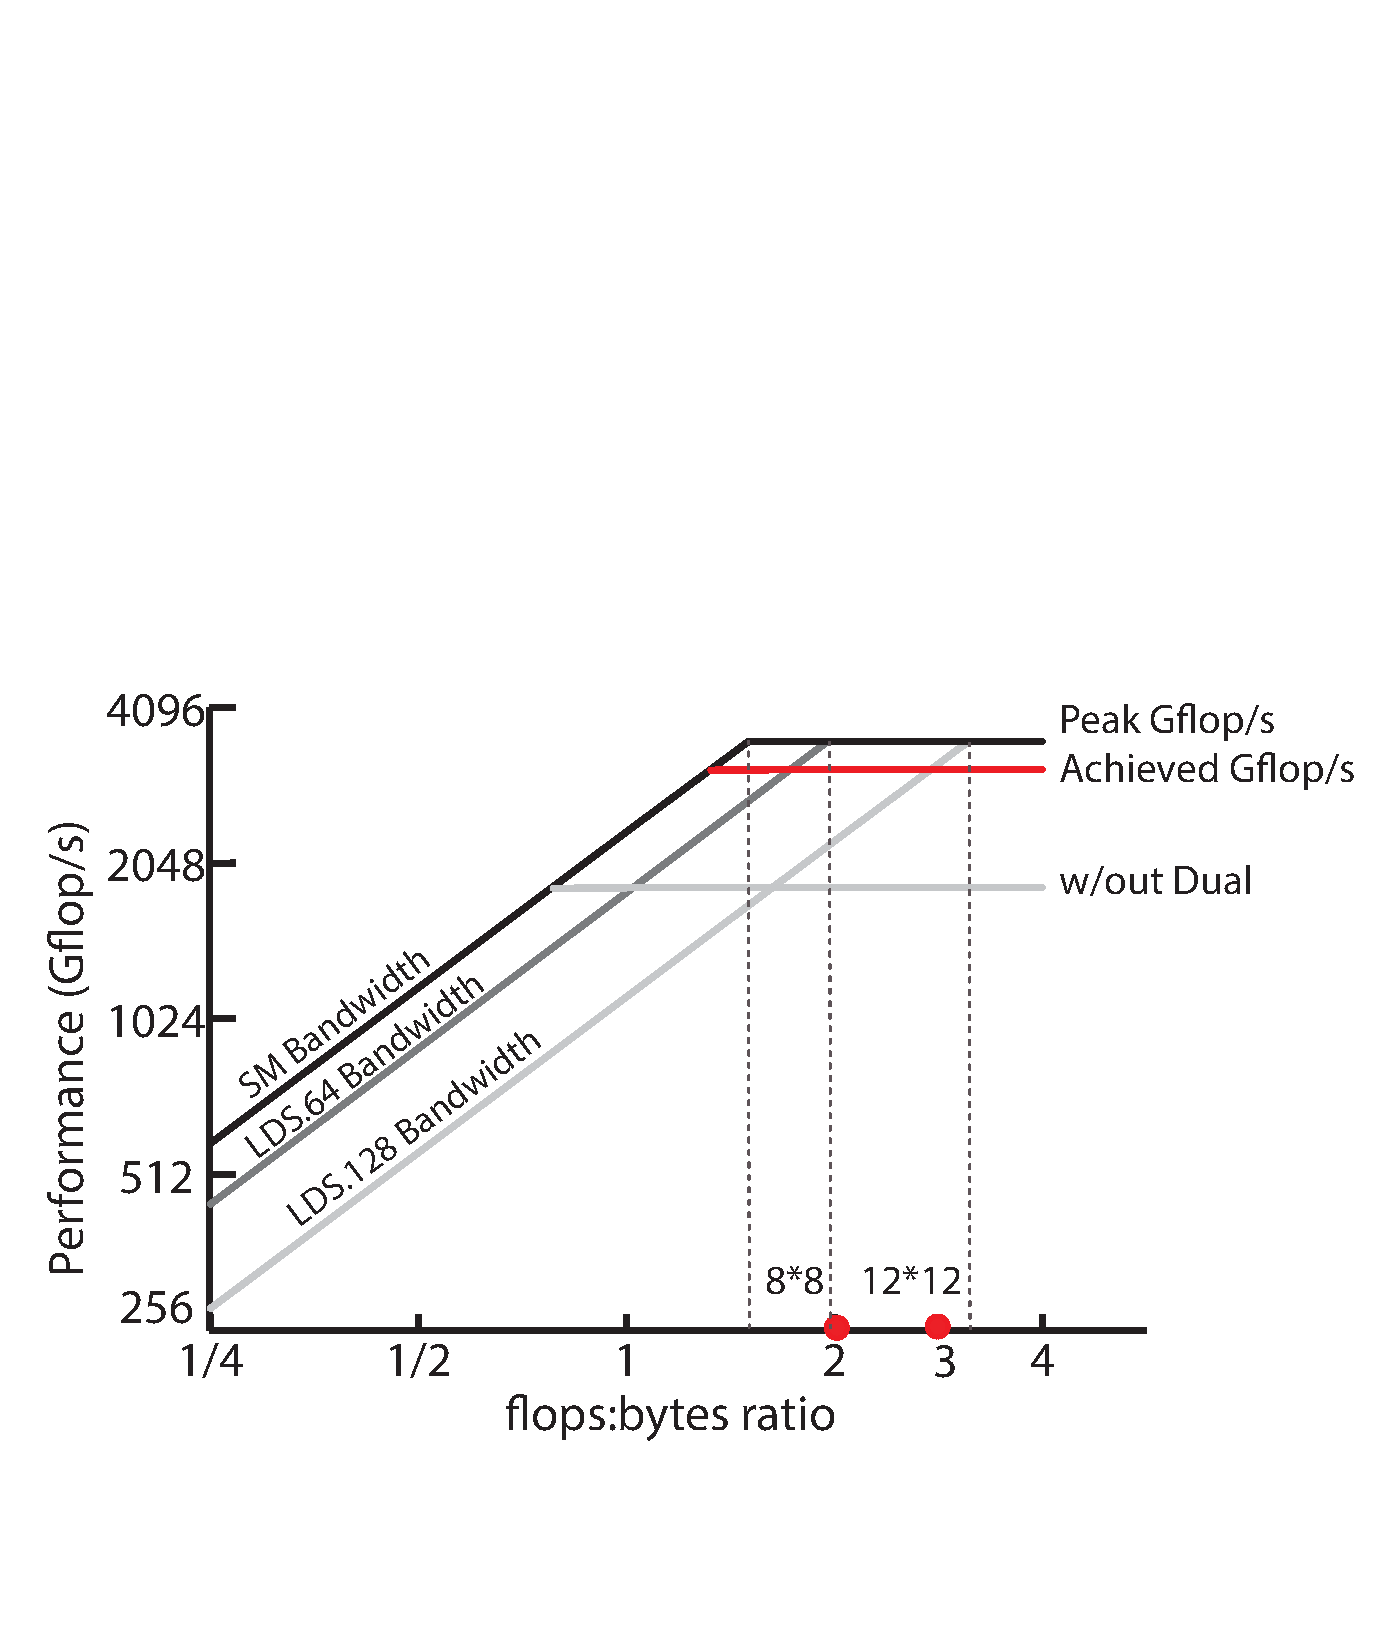
\includegraphics[scale=0.32]{roofline_sm}
    \caption{Shared memory roofline model using log-log scale. ``SM Bandwidth'' means shared memory's theoretical
    bandwidth. }% Horizontal lines shows different Gflops.}
\label{fig:roofline_shared}
\end{center}
\end{figure}

\subsubsection{Upper Bound Analysis}


We estimate the upper bound factors: {\tt LDS}, {\tt LDG} and {\tt FFMA} which correspond to three kinds of resources respectively, 
shared
memory, global memory, and computation power. In the register blocking loop, each thread block computes $b_m*b_n*b_k$ and reads $b_m*b_k+b_n*b_k$ words. The upper bound of global memory bandwidth can be modeled as:
\begin{equation}
    \frac{2*b_m*b_n*b_k}{4*(b_m*b_k + b_n*b_k)} = \frac{Gflop/s}{bandwidth}
    \label{equ:global}
\end{equation}
According to parameters in our SGEMM implementation, $b_m=b_n=192$, $b_k=4$, $Gflop/s=3520$, so $73$ GB/s is the minimal
requirement for global memory bandwidth in order to achieve the theoretical peak $3520$ Gflops.
For shared memory, inside each loop, $(r_x*b_k + r_y * b_k)*t_x*t_y$ words will be read from shared memory, in which $t_x$ and
$t_y$ are thread blocking dimensions, $r_x$ and $r_y$ are register blocking sizes. The computation is $b_m*b_n*b_k$. Based on the ratio of computation to shared memory access,
\begin{equation}
    \frac{2*b_m*b_k*b_n}{4*t_x*t_y*(r_x*b_k + r_y *b_k)}  = \frac{Gflop/s}{bandwidth}
    \label{equ:shared}
\end{equation}


For Kepler GPU the minimum bandwidth requirement for shared memory is $1173$GB/s, and the bandwidth requirement is
$1173/13=90$ GB/s for each SM. The hardware provides $200$GB/s global memory bandwidth and $2349$GB/s shared memory bandwidth in theory, which are higher than requirements, and hence neither the bandwidth of shared nor global memory will be the bottleneck.

SGEMM has different computation to memory access ratio in terms of global memory and shared memory, so we demonstrate
two roofline models in Figure~\ref{fig:roofline_global} and~\ref{fig:roofline_shared}. 
The slope of slant line in Figure~\ref{fig:roofline_global} is global memory bandwidth. The x-axis is computation to global
memory access ratio of an algorithm. 
By Equation~\ref{equ:global}, the flops:bytes ratio of $192\times192$ and $128\times128$ shared 
memory blocking of SGEMM are $48$ and $32$ respectively. The horizontal lines show machine's peak performance, our SGEMM
achieved performance, and its performance without dual issue.
This figure demonstrates that SGEMM is not global memory bounded for both $128\times128$ and $192\times 192$ shared memory blockings.
The slope of slant line in Figure~\ref{fig:roofline_shared} is the bandwidth of shared memory. The x-axis is computation to
shared memory access ratio of an algorithm. 
By Equation~\ref{equ:shared}, the flops:bytes ratio of $12\times12$, $8\times8$ register blocking SGEMM are $3$ and $2$ respectively. 
This figure shows SGEMM is not bounded by shared memory through our {\tt LDS} optimization. 
However, if we use {\tt LDS.128} instead of {\tt LDS.64}, SGEMM will be bounded by shared memory even for $12\times 12$ blocking.

The loss of peak performance can be explained by the following reasons. As we have shown in 
section~\ref{sec:assembler}, {\tt FFMA} throughput can achieve $97.67\%$. 
The loss is about $2.33\%$, which may come 
from the overhead of warp scheduler in {\tt FFMA} dual issue mode. The double-buffering algorithm can amortize the latency 
of {\tt LDS}.
With $12\times12$ register blocking and $4$ times unrolling, there will be $144*4=576$ {\tt FFMA}s in the loop.
With our designed {\tt FFMA} dual issue pattern, every six {\tt FFMA}s needs four clock cycles in the pipeline.
It needs $4\times144\times4/6=384$ clocks for each thread, two {\tt LDG.128}s are needed.
We observe each {\tt LDG} has $10$ clocks penalty, the total {\tt LDG} will cause $2\times10/384 = 5.2\%$ loss. Other
penalties come from synchronization and writing $C$ matrix in the block.
